\section{Defense Strategies} \label{sec:defense}

%%%%%%%%%%%%%%%%%%%%%%%%%%%%%%%%%%%%%%%%%%%%%%%
%%%%%  Rethink the security and defense
%%%%%. 1. Do no share original gradient
%%%%%. 2. Do no share all gradients
%%%%%%%%%%%%%%%%%%%%%%%%%%%%%%%%%%%%%%%%%%%%%%%%
% As demonstrated in experiments, DLG is able to perform record-level revealing from the shared gradients. This sets a new challenge to existing multi-node learning frameworks. In this section, we discuss some possible strategies for defense.

\subsection{Noisy Gradients} \label{sec:defense:noisy}
One straightforward attempt to defense DLG is to add noise on gradients before sharing. 
% 
% This action has been empirically proved that only has little effects on performance, however, will make the DLG side optimization difficult.  
% 
To evaluate, we experiment  Gaussian and Laplacian noise (widely used in differential privacy studies) distributions with variance range from $10^{-1}$ to $10^{-4}$ and central $0$. From Fig.~\ref{fig:defense:gaussian} and \ref{fig:defense:Laplacian}, we observe that the defense effect mainly depends on the magnitude of distribution variance and less related to the noise types. When variance is at the scale of $10^{-4}$, the noisy gradients do not prevent the leak. For noise with variance $10^{-3}$, though with artifacts, the leakage can still be performed. Only when the variance is larger than $10^{-2}$ and the noise is starting affect the accuracy, DLG will fail to execute and Laplacian tends to slight better at scale $10^{-3}$. However, noise with variance larger than $10^{-2}$ will degrade the accuracy significantly (Tab.~\ref{tab:defense_vs_accuracy}).

Another common perturbation on gradients is half precision, which was initially designed to save GPU memory footprints and also widely used to reduce communication bandwidth. We test two popular half precision implementations IEEE float16 (\textit{Single-precision floating-point format}) and bfloat16 (\textit{Brain Floating Point}~\cite{tagliavini2017transprecision}, a truncated version of 32 bit float). Shown in Fig.~\ref{fig:defense:fp16},  both half precision formats fail to protect the training data. We also test another popular low-bit representation Int-8. Though it successfully prevents the leakage, the performance of model drops seriously (Tab.~\ref{tab:defense_vs_accuracy}).

\newcommand{\lgcmark}{\textcolor{green}{\cmark}}
\newcommand{\lgxmark}{\textcolor{red}{\xmark}}

\begin{figure}[t]
    \centering
    % 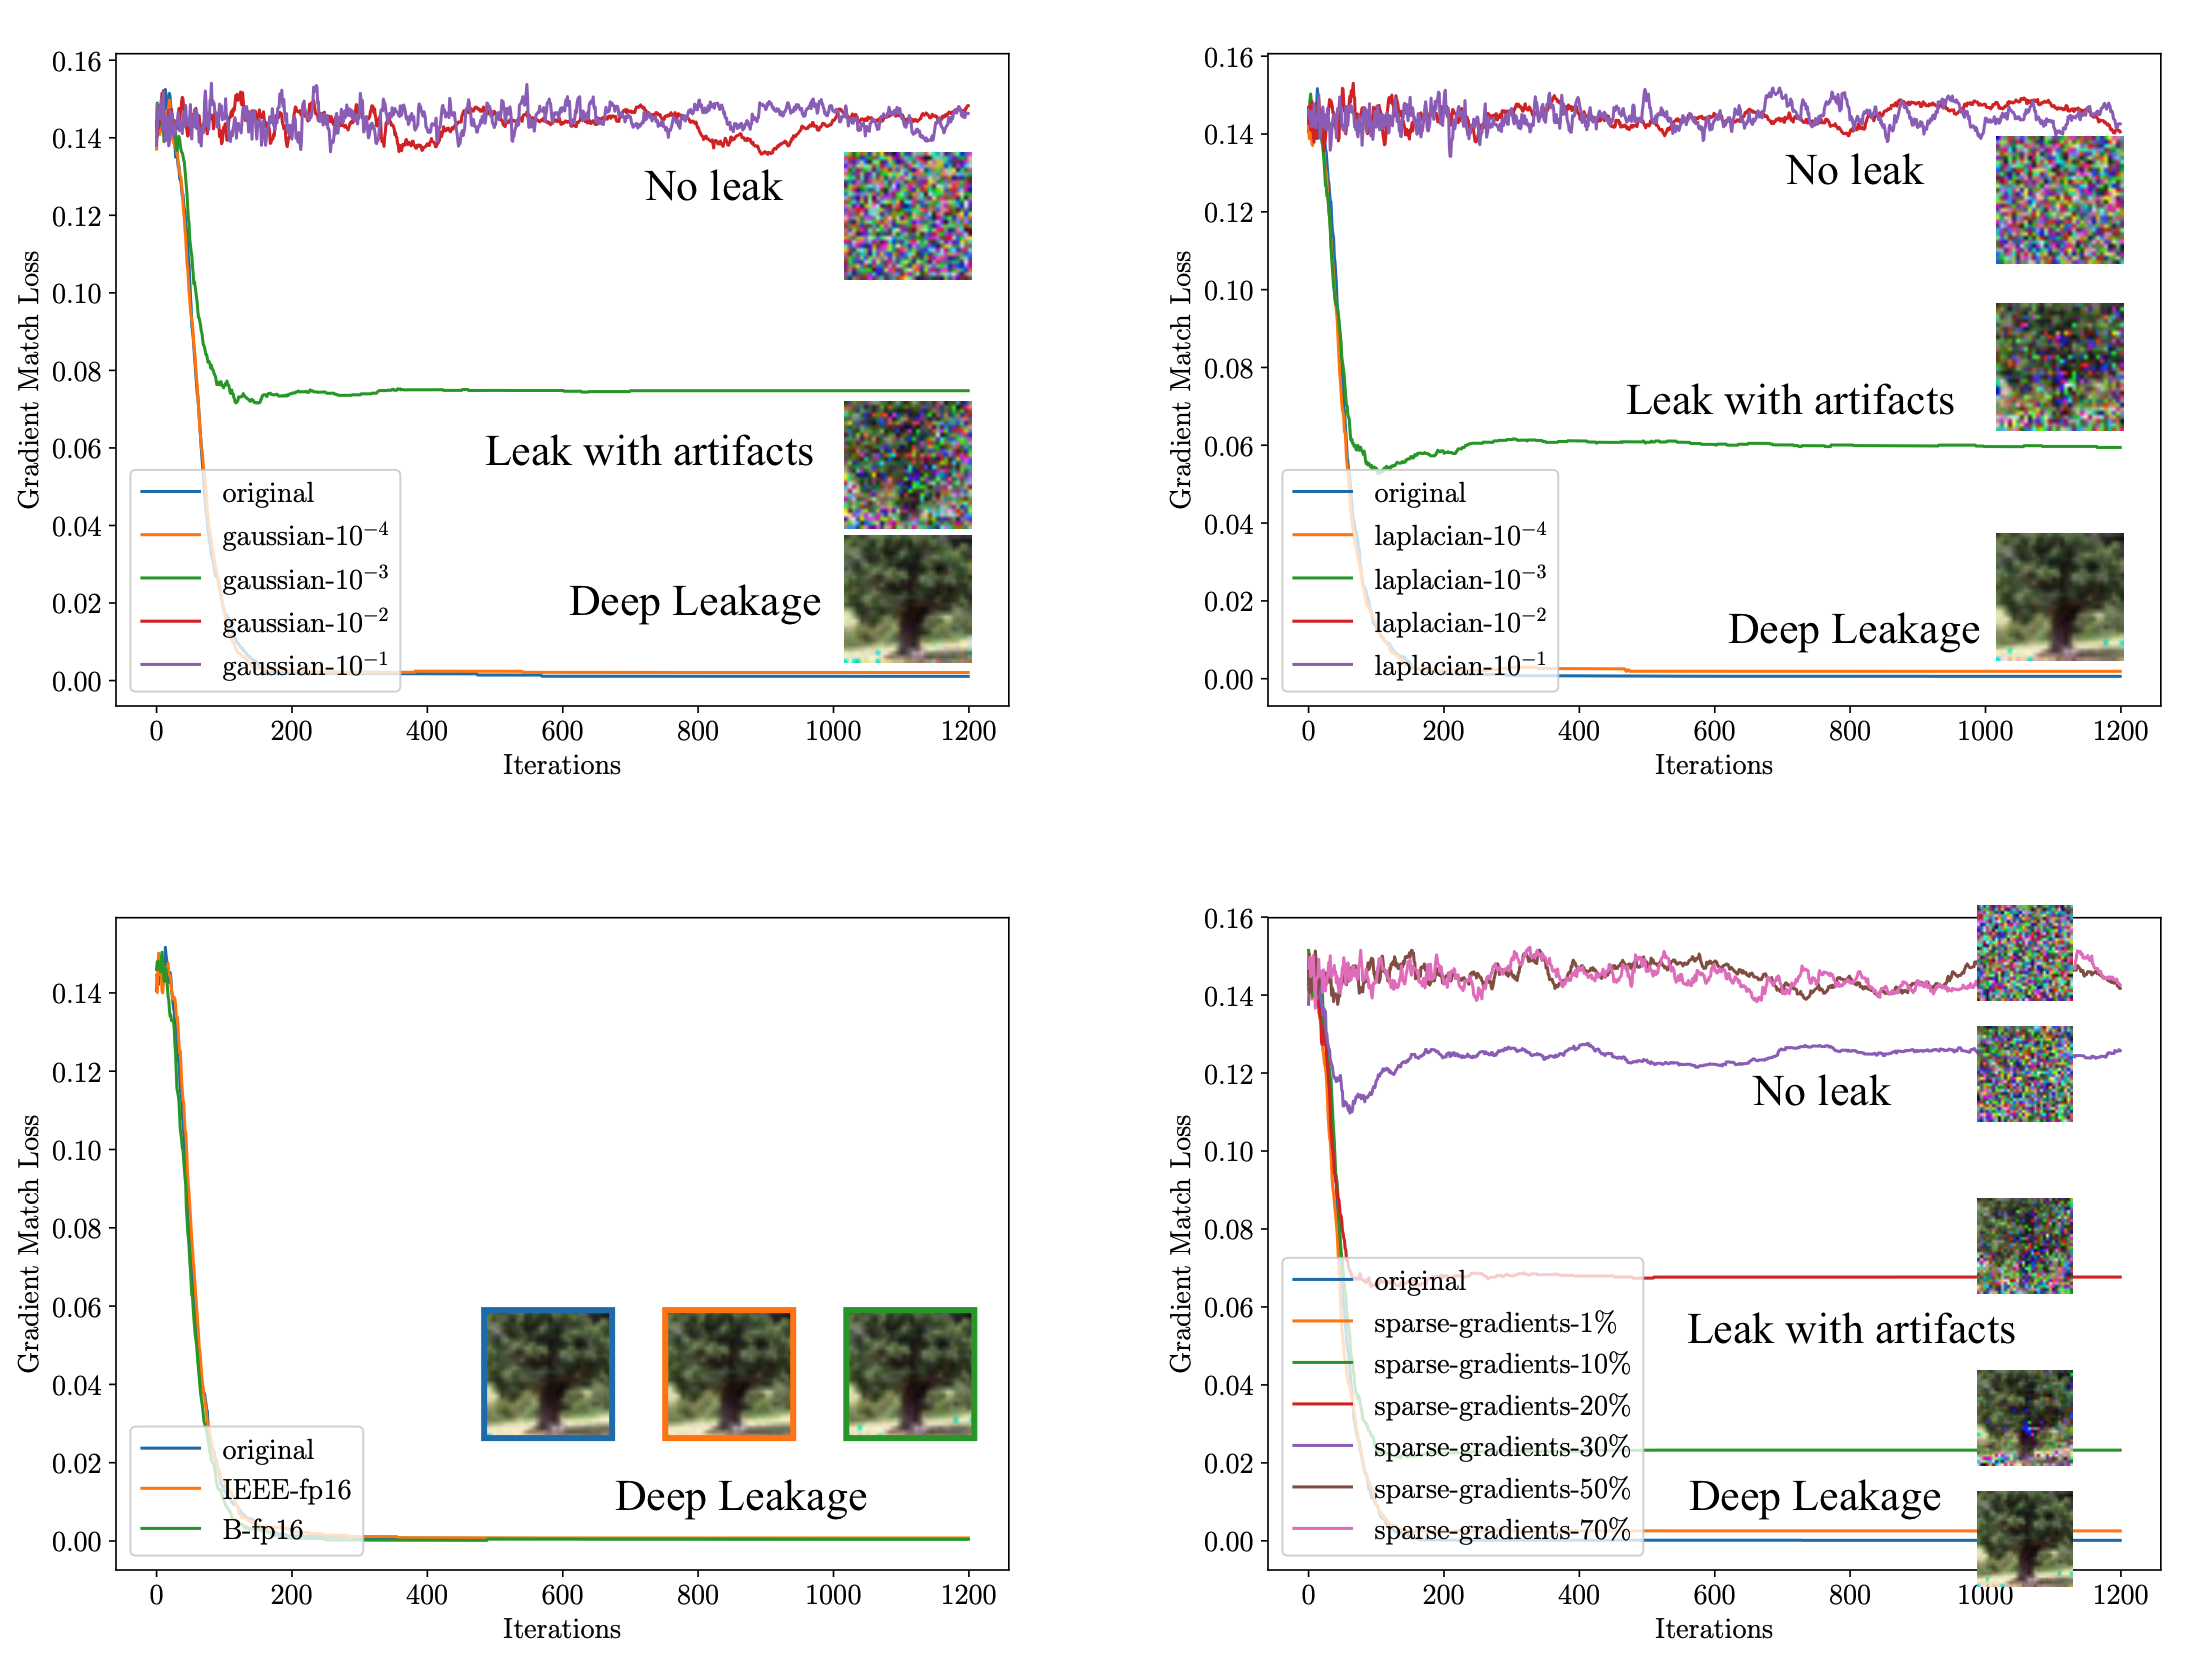
\includegraphics[width=\linewidth]{figures/fig4}
    % \caption{Caption \SH{font size should be as large as main text; reduce the space between the two rows}}
    \centering
    \begin{subfigure}[b]{0.49\textwidth}
        \centering
        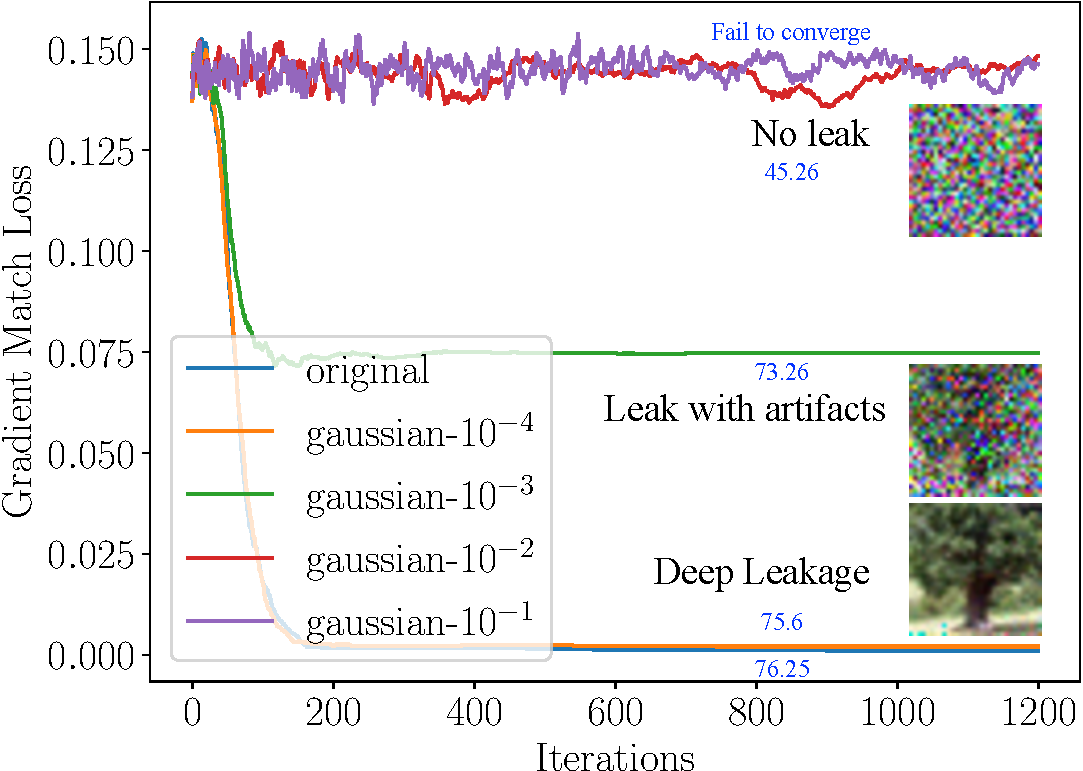
\includegraphics[width=\textwidth]{figures/fig5_gaussian-crop.pdf}
        \caption{Defend with different magnitude Gaussian noise.}
        \label{fig:defense:gaussian}
    \end{subfigure}
    \begin{subfigure}[b]{0.49\textwidth}
        \centering
        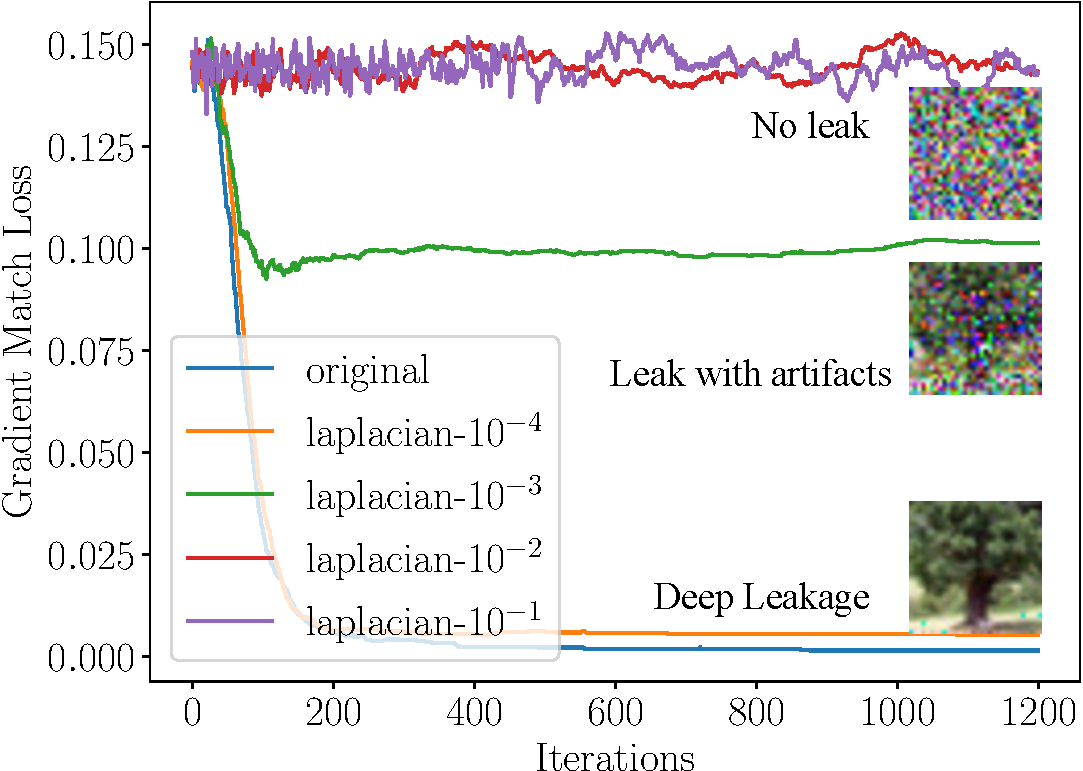
\includegraphics[width=\textwidth]{figures/fig5_laplacian-crop.pdf}
        \caption{Defend with different magnitude Laplacian noise.}
        \label{fig:defense:Laplacian}
    \end{subfigure} 
    \\ \vspace{4pt}
    \begin{subfigure}[b]{0.49\textwidth}
        \centering
        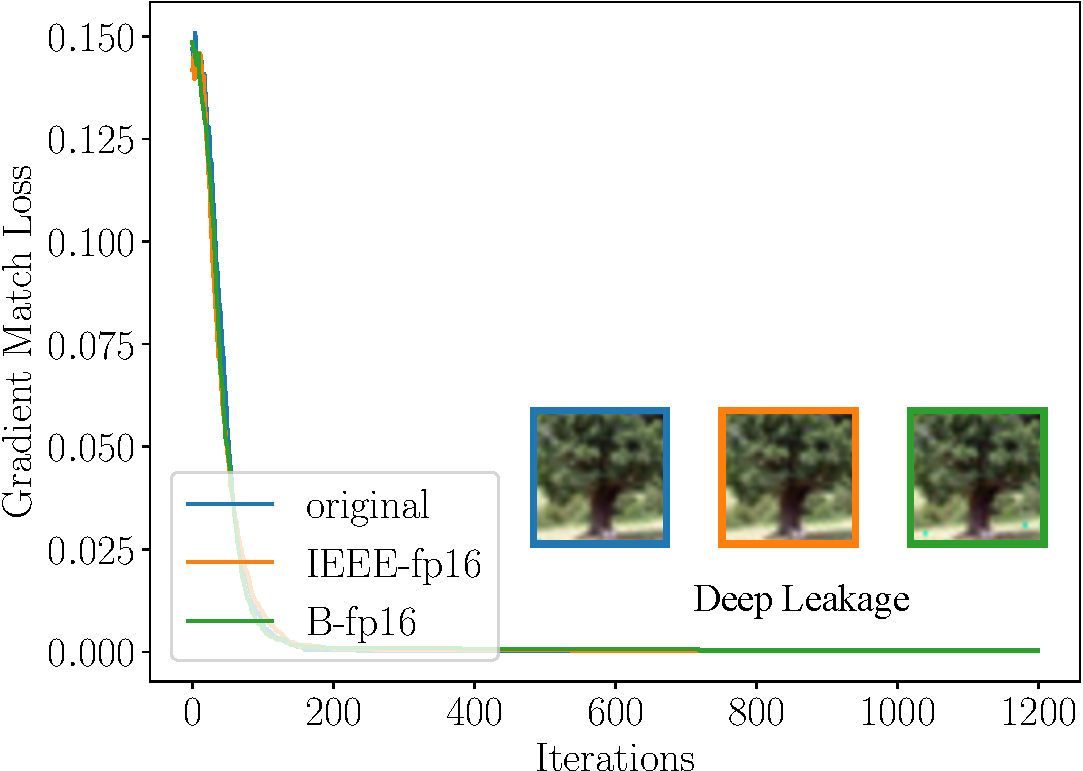
\includegraphics[width=\textwidth]{figures/fig5_fp16-crop.pdf}
        \caption{Defend with fp16 convertion.}
        \label{fig:defense:fp16}
    \end{subfigure}
    \begin{subfigure}[b]{0.49\textwidth}
        \centering
        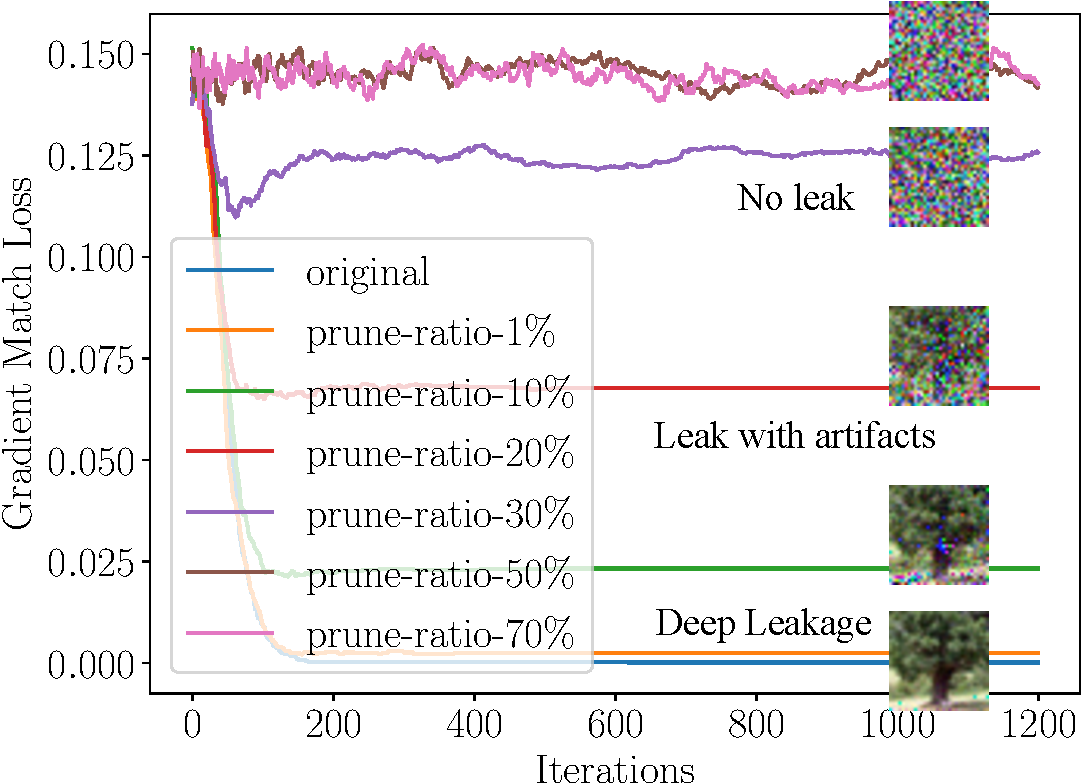
\includegraphics[width=\textwidth]{figures/fig5_dgc-crop.pdf}
        \caption{Defend with gradient pruning.}
        \label{fig:defense:dgc}
    \end{subfigure} 
    \caption{The effectiveness of various defense strategies. }
    \label{fig:defense}
    \vspace{-5pt}
\end{figure}
% 
\begin{table}[t]
\setlength{\tabcolsep}{3.5pt}
\centering
\footnotesize{
\begin{tabular}[t]{c||c||c|c|c|c||c|c|c|c||c}
    & Original  & \textbf{G}-$10^{-4}$ & \textbf{G}-$10^{-3}$ & \textbf{G}-$10^{-2}$ & \textbf{G}-$10^{-1}$  & \textbf{FP}-16  \\ \hline
    Accuracy & 76.3\% & 75.6\% & 73.3\% & 45.3\% & $\le$1\% & 76.1\% \\ \hline
    Defendability & -- & \lgxmark &  \lgxmark & \lgcmark &  \lgcmark & \lgxmark \\ \hline
    % 
    &     & \textbf{L}-$10^{-4}$ & \textbf{L}-$10^{-3}$ & \textbf{L}-$10^{-2}$ & \textbf{L}-$10^{-1}$  & \textbf{Int}-8  \\ \hline
    Accuracy & -- & 75.6\% & 73.4\% & 46.2\% & $\le$1\% & 53.7\% \\ \hline
    Defendability & -- & \lgxmark &  \lgxmark & \lgcmark &  \lgcmark & \lgcmark \\
\end{tabular}
}
\caption{The trade-off between accuracy and defendability. \textbf{G}: Gaussian noise, \textbf{L}: Laplacian noise, \textbf{FP}: Floating number, \textbf{Int}: Integer quantization.
\lgcmark~means it successfully defends against DLG while \lgxmark~means fails to defend (whether the results are visually recognizable). The accuracy is evaluated on CIFAR-100.
}
\label{tab:defense_vs_accuracy}
\vspace{-10pt}
\end{table}
\subsection{Gradient Compression and Sparsification} \label{sec:defense:few_gradients}
% Beside perturbing the gradients, another defense approach is to sparsify the gradients~\cite{DGC}, an effective  
We next experimented to defend by gradient compression~\cite{lin2017deep, tsuzuku2018variance}: Gradients with small magnitudes are pruned to zero. It's more difficult for DLG to match the gradients as the optimization targets are pruned.
% 
We evaluate how different level of sparsities (range from 1\% to 70\%) defense the leakage. When sparsity is 1\% to 10\%, it has almost no effects against DLG. When prune ratio increases to 20\%, as shown in Fig.~\ref{fig:defense:dgc}, there are obvious artifact pixels on the recover images.  
% 
We notice that maximum tolerance of sparsity is around 20\%. 
When pruning ratio is larger, the recovered images are no longer visually recognizable and thus gradient compression successfully prevents the leakage.

Previous work~\cite{tsuzuku2018variance, lin2017deep} show that gradients can be compressed by more than 300$\textbf{}\times$ without losing accuracy by error compensation techniques. In this case, the sparsity is above 99\% and already exceeds the maximum tolerance of DLG (which is around 20\%). It suggests that compressing the gradients is a practical approach to avoid the deep leakage. 

\subsection{Large Batch, High Resolution and Cryptology}\label{sec:defend:others}

If changes on training settings are allowed, then there are more defense strategies. As suggested in Tab.~\ref{tab:batched_restore}, increasing the batch size makes the leakage more difficult because there are more variables to solve during optimization. 
% 
Following the idea, upscaling the input images can be also a good defense, though some changes on CNN architectures is required. 
% 
According to our experiments, DLG currently only works for batch size up to 8 and image resolution up to 64$\times$64. 

Beside methods above, cryptology can be also used to prevent the leakage: Bonawitz~\etal~\cite{bonawitz16secure_Aggregation} designs a secure aggregation protocols and Phong~\etal~\cite{phong2018privacy} proposes to encrypt the gradients before sending. Among all defenses, cryptology is the most secured one. However, both methods have their limitations and not general enough: secure aggregation~\cite{bonawitz16secure_Aggregation} requires gradients to be integers thus not compatible with most CNNs, and homomorphic encryption~\cite{phong2018privacy} is against parameter server only. 

\section{Conclusions}

In this paper, we introduce the \emph{Deep Leakage from Gradients} (DLG): an algorithm that can obtain the local training data from public shared gradients. 
% 
DLG does not rely on any generative model or extra prior about the data. Our experiments on vision and language tasks both demonstrate the critical risks of such deep leakage and show that such deep leakage can be only prevented when defense strategies starts to degrade the accuracy.
%
% Though with some limitations (discussed in Sec.~\ref{sec:defend:others}),
This sets a challenge to modern multi-node learning system (e.g., distributed training, federated learning).
% 
We hope this work would raise people's awareness about the security of gradients and bring the community to rethink the safety of existing gradient sharing scheme. 

% which brings a new challenge to the modern multi-node learning system. We discuss possible methods to defense again this attack.
% It is worth noting that, though we only tested on two models, DLG can be extended to more popular machine learning models as the attack only requires the model to be differentiable. 
% Experiments across two popular tasks demonstrate the effectiveness of our algorithm and we also discuss possible methods to defense again this attack.

\section*{Acknowledgments}

We sincerely thank MIT-IBM Watson AI lab, Intel, Facebook and AWS for supporting this work. We sincerely thank John Cohn for the discussions. 

% \newpage
